\begin{center}
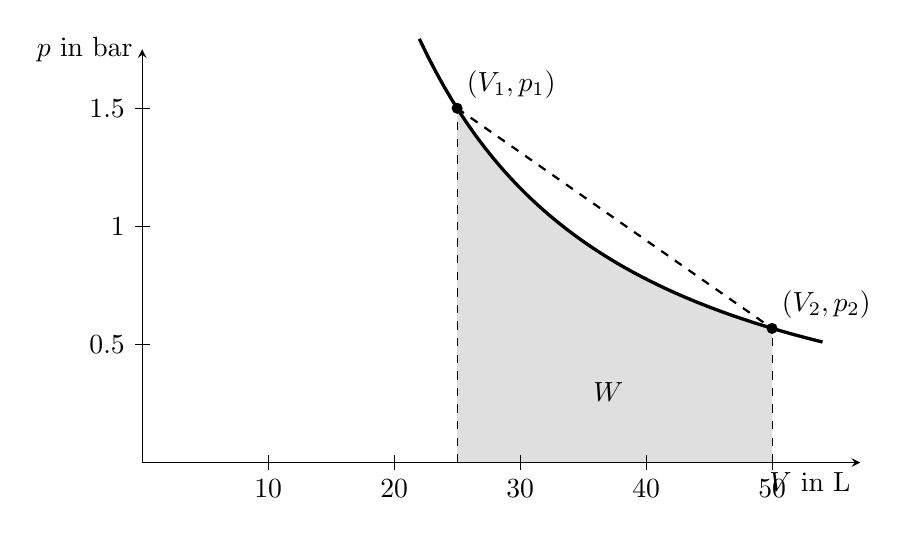
\begin{tikzpicture}[>=stealth, x=0.16cm, y=3cm]
 \fill[gray!25] (25,0) -- plot[domain=25:50, samples=40] (\x,{1.5*(25/\x)^1.4}) -- (50,0) -- cycle;
 \draw[->] (0,0) -- (57,0) node[below left] {$V$ in L};
 \draw[->] (0,0) -- (0,1.75) node[left] {$p$ in bar};
 \foreach \vl in {10,20,30,40,50} \draw (\vl,0.03) -- (\vl,-0.03) node[below] {\vl};
 \foreach \pl in {0.5,1,1.5} \draw (0.6,\pl) -- (-0.6,\pl) node[left] {\pl};
 \draw[very thick] plot[domain=22:54, samples=50] (\x,{1.5*(25/\x)^1.4});
 \draw[thick, dashed] (25,1.5) -- (50,0.568);
 \draw[dashed] (25,0) -- (25,1.5);
 \draw[dashed] (50,0) -- (50,0.568);
 \fill (25,1.5) circle (2pt) node[above right] {$(V_1, p_1)$};
 \fill (50,0.568) circle (2pt) node[above right] {$(V_2, p_2)$};
 \node at (37,0.3) {$W$};
\end{tikzpicture}
\end{center}

\begin{abcliste}
\abc Mit $p\,V^{7/5} = p_1V_1^{7/5}$ ist der Druck während der Expansion
\begin{align}
 p(V) &= p_1\left(\frac{V_1}{V}\right)^{7/5}
\end{align}
Die vom Gas verrichtete Arbeit ist die Fläche unter dieser Kurve zwischen $V_1 = \VaO$ und $V_2 = 2\,V_1$ (grau). Der Taschenrechner (numerische Integration) gibt
\begin{align}
 W &= \int_{V_1}^{V_2} p_1\left(\frac{V_1}{V}\right)^{7/5}\mathrm{d}V = \WadF \\
   &= \frac{5}{2}\cdot\pa\cdot\Va\cdot\left(1-\left(\frac{1}{2}\right)^{2/5}\right) \\
   &= \Wad \approx \result{\WadP{3}{2}}
\end{align}
Dasselbe folgt aus dem ersten Hauptsatz: Ohne Wärmeaustausch ist $W = -\Delta U = \frac{5}{2}\left(p_1V_1-p_2V_2\right)$.

\abc Der Enddruck ist
\begin{align}
 p_2 &= \pbF = \pa\cdot\left(\frac{1}{2}\right)^{7/5} = \pb \approx \pbbP{0}{2}
\end{align}
Die Fläche unter der Geraden (Trapez) ist
\begin{align}
 W_\text{lin} &= \WliF \\
   &= \frac{\pa+\pb}{2}\cdot\left(\Vb-\Va\right) \\
   &= \Wli \approx \result{\WliP{3}{2}}
\end{align}
Weil die Adiabate nach unten gewölbt ist, liegt die Gerade über der Kurve; die Näherung ist um etwa \dWrP{0}{2} zu gross.
\end{abcliste}
